\section{Analyzer::Base$<$ W $>$ Class Template Reference}
\label{classAnalyzer_1_1Base}\index{Analyzer::Base@{Analyzer::Base}}
{\tt \#include $<$analyzerbase.h$>$}

Inheritance diagram for Analyzer::Base$<$ W $>$:\begin{figure}[H]
\begin{center}
\leavevmode
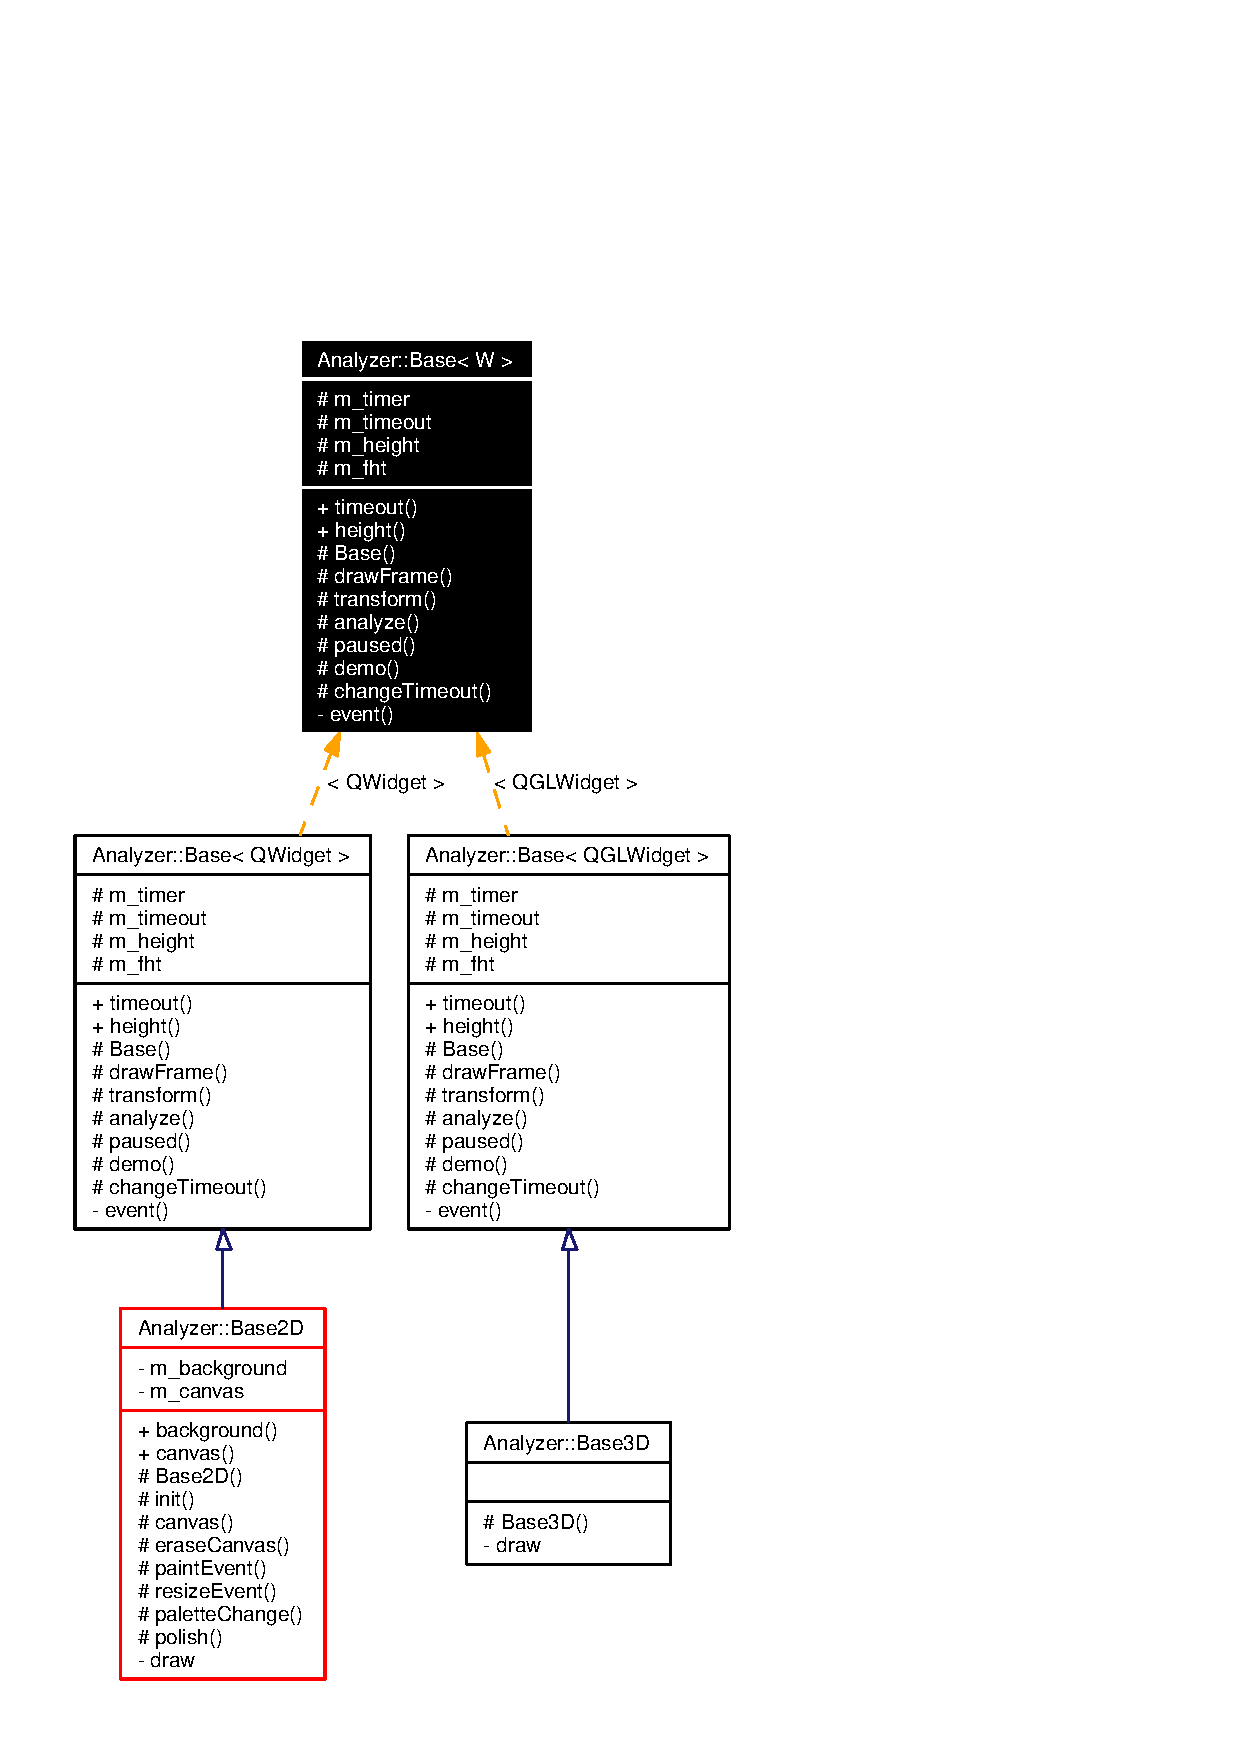
\includegraphics[width=175pt]{classAnalyzer_1_1Base__inherit__graph}
\end{center}
\end{figure}
Collaboration diagram for Analyzer::Base$<$ W $>$:\begin{figure}[H]
\begin{center}
\leavevmode
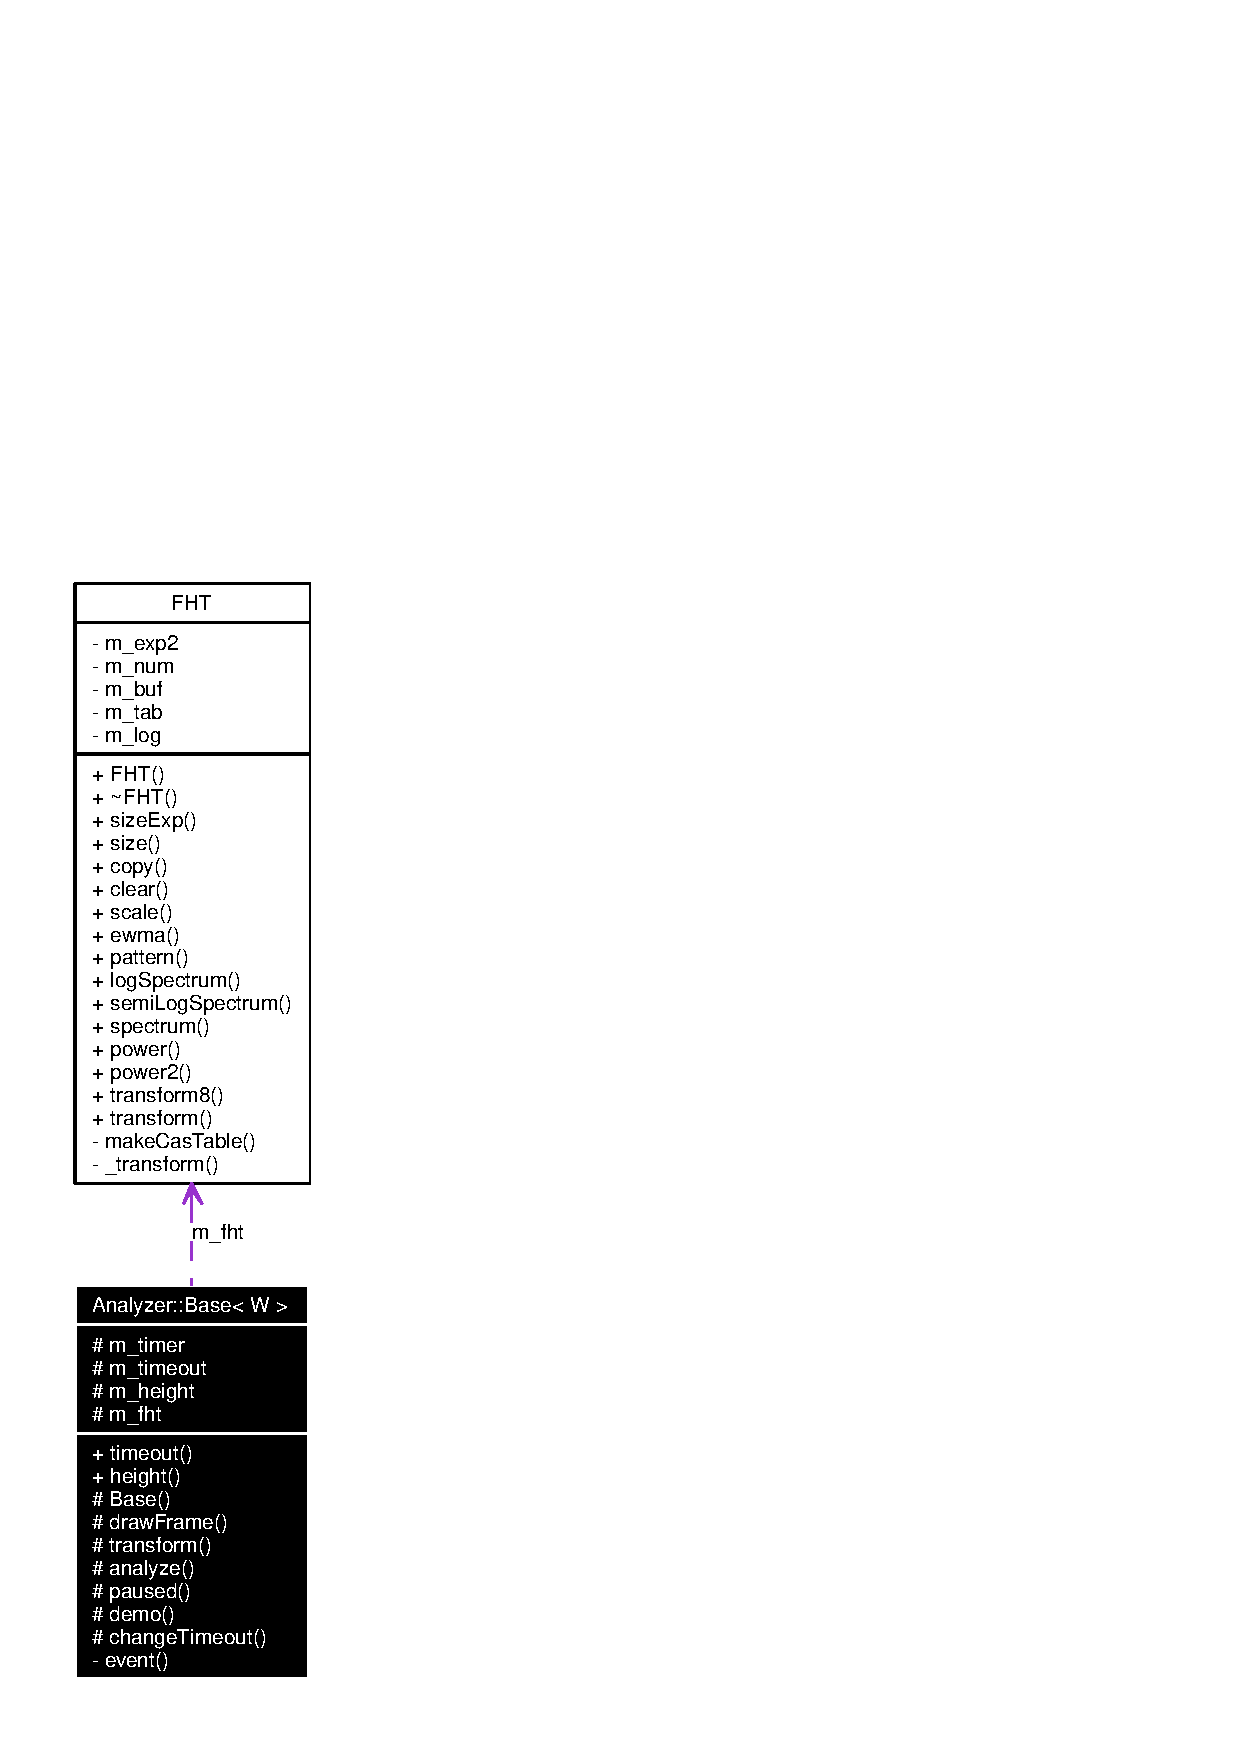
\includegraphics[width=74pt]{classAnalyzer_1_1Base__coll__graph}
\end{center}
\end{figure}
\subsubsection*{template$<$class W$>$ class Analyzer::Base$<$ W $>$}

\subsection*{Public Member Functions}
\begin{CompactItemize}
\item 
uint {\bf timeout} () const 
\item 
uint {\bf height} () const 
\end{CompactItemize}
\subsection*{Protected Member Functions}
\begin{CompactItemize}
\item 
{\bf Base} ({\bf QWidget} $\ast$, uint, uint=7)
\item 
void {\bf draw\-Frame} ()
\item 
virtual void {\bf transform} ({\bf Scope} \&)
\item 
virtual void {\bf analyze} (const {\bf Scope} \&)=0
\item 
virtual void {\bf paused} ()
\item 
virtual void {\bf demo} ()
\item 
void {\bf change\-Timeout} (uint new\-Timeout)
\end{CompactItemize}
\subsection*{Protected Attributes}
\begin{CompactItemize}
\item 
QTimer {\bf m\_\-timer}
\item 
uint {\bf m\_\-timeout}
\item 
uint {\bf m\_\-height}
\item 
{\bf FHT} {\bf m\_\-fht}
\end{CompactItemize}
\subsection*{Private Member Functions}
\begin{CompactItemize}
\item 
bool {\bf event} (QEvent $\ast$)
\end{CompactItemize}


\subsection{Constructor \& Destructor Documentation}
\index{Analyzer::Base@{Analyzer::Base}!Base@{Base}}
\index{Base@{Base}!Analyzer::Base@{Analyzer::Base}}
\subsubsection{\setlength{\rightskip}{0pt plus 5cm}template$<$class W$>$ {\bf Analyzer::Base}$<$ W $>$::{\bf Base} ({\bf QWidget} $\ast$, uint, uint = 7)\hspace{0.3cm}{\tt  [protected]}}\label{classAnalyzer_1_1Base_Analyzer_1_1Baseb0}




Definition at line 43 of file analyzerbase.cpp.



\footnotesize\begin{verbatim}44   : W( parent )
45   , m_timeout( timeout )
46   , m_height( 0 )
47   , m_fht( scopeSize )
48 {}
\end{verbatim}\normalsize 


\subsection{Member Function Documentation}
\index{Analyzer::Base@{Analyzer::Base}!analyze@{analyze}}
\index{analyze@{analyze}!Analyzer::Base@{Analyzer::Base}}
\subsubsection{\setlength{\rightskip}{0pt plus 5cm}template$<$class W$>$ virtual void {\bf Analyzer::Base}$<$ W $>$::analyze (const {\bf Scope} \&)\hspace{0.3cm}{\tt  [protected, pure virtual]}}\label{classAnalyzer_1_1Base_Analyzer_1_1Baseb3}




Implemented in {\bf Sonogram} {\rm (p.\,\pageref{classSonogram_Sonograma3})}.

Referenced by Analyzer::Base$<$ W $>$::demo(), and Analyzer::Base$<$ W $>$::draw\-Frame().\index{Analyzer::Base@{Analyzer::Base}!changeTimeout@{changeTimeout}}
\index{changeTimeout@{changeTimeout}!Analyzer::Base@{Analyzer::Base}}
\subsubsection{\setlength{\rightskip}{0pt plus 5cm}template$<$class W$>$ void {\bf Analyzer::Base}$<$ W $>$::change\-Timeout (uint {\em new\-Timeout})\hspace{0.3cm}{\tt  [inline, protected]}}\label{classAnalyzer_1_1Base_Analyzer_1_1Baseb6}




Definition at line 54 of file analyzerbase.h.



\footnotesize\begin{verbatim}55     {
56         m_timer.changeInterval( newTimeout );
57         m_timeout = newTimeout;
58     }
\end{verbatim}\normalsize 
\index{Analyzer::Base@{Analyzer::Base}!demo@{demo}}
\index{demo@{demo}!Analyzer::Base@{Analyzer::Base}}
\subsubsection{\setlength{\rightskip}{0pt plus 5cm}template$<$class W$>$ void {\bf Analyzer::Base}$<$ W $>$::demo ()\hspace{0.3cm}{\tt  [protected, virtual]}}\label{classAnalyzer_1_1Base_Analyzer_1_1Baseb5}




Reimplemented in {\bf Sonogram} {\rm (p.\,\pageref{classSonogram_Sonograma5})}.

Definition at line 128 of file analyzerbase.cpp.

References Analyzer::Base$<$ W $>$::analyze(), and Analyzer::Scope.

Referenced by Analyzer::Base$<$ W $>$::draw\-Frame().



\footnotesize\begin{verbatim}129 {
130     static int t = 201; //FIXME make static to namespace perhaps
131 
132     if( t > 999 ) t = 1; //0 = wasted calculations
133     if( t < 201 )
134     {
135         Scope s( 32 );
136 
137         const double dt = double(t) / 200;
138         for( uint i = 0; i < s.size(); ++i )
139             s[i] = dt * (sin( M_PI + (i * M_PI) / s.size() ) + 1.0);
140 
141         analyze( s );
142     }
143     else analyze( Scope( 32, 0 ) );
144 
145     ++t;
146 }
\end{verbatim}\normalsize 


Here is the call graph for this function:\begin{figure}[H]
\begin{center}
\leavevmode

\includegraphics[width=157pt]{classAnalyzer_1_1Base_Analyzer_1_1Baseb5_cgraph}
\end{center}
\end{figure}
\index{Analyzer::Base@{Analyzer::Base}!drawFrame@{drawFrame}}
\index{drawFrame@{drawFrame}!Analyzer::Base@{Analyzer::Base}}
\subsubsection{\setlength{\rightskip}{0pt plus 5cm}template$<$class W$>$ void {\bf Analyzer::Base}$<$ W $>$::draw\-Frame ()\hspace{0.3cm}{\tt  [protected]}}\label{classAnalyzer_1_1Base_Analyzer_1_1Baseb1}




Definition at line 94 of file analyzerbase.cpp.

References Analyzer::Base$<$ W $>$::analyze(), Analyzer::Base$<$ W $>$::demo(), Engine\-Controller::engine(), Analyzer::Base$<$ W $>$::paused(), Engine\-Base::scope(), Analyzer::Scope, Engine\-Base::state(), and Analyzer::Base$<$ W $>$::transform().



\footnotesize\begin{verbatim}95 {
96     EngineBase *engine = EngineController::engine();
97 
98     switch( engine->state() )
99     {
100     case EngineBase::Playing:
101     {
102         Scope *scope = engine->scope();
103 
104         if( !scope->empty() )
105         {
106             transform( *scope );
107             analyze( *scope );
108         }
109 
110         delete scope;
111 
112         break;
113     }
114     case EngineBase::Paused:
115         paused();
116         break;
117 
118     default:
119         demo();
120     }
121 }
\end{verbatim}\normalsize 


Here is the call graph for this function:\begin{figure}[H]
\begin{center}
\leavevmode
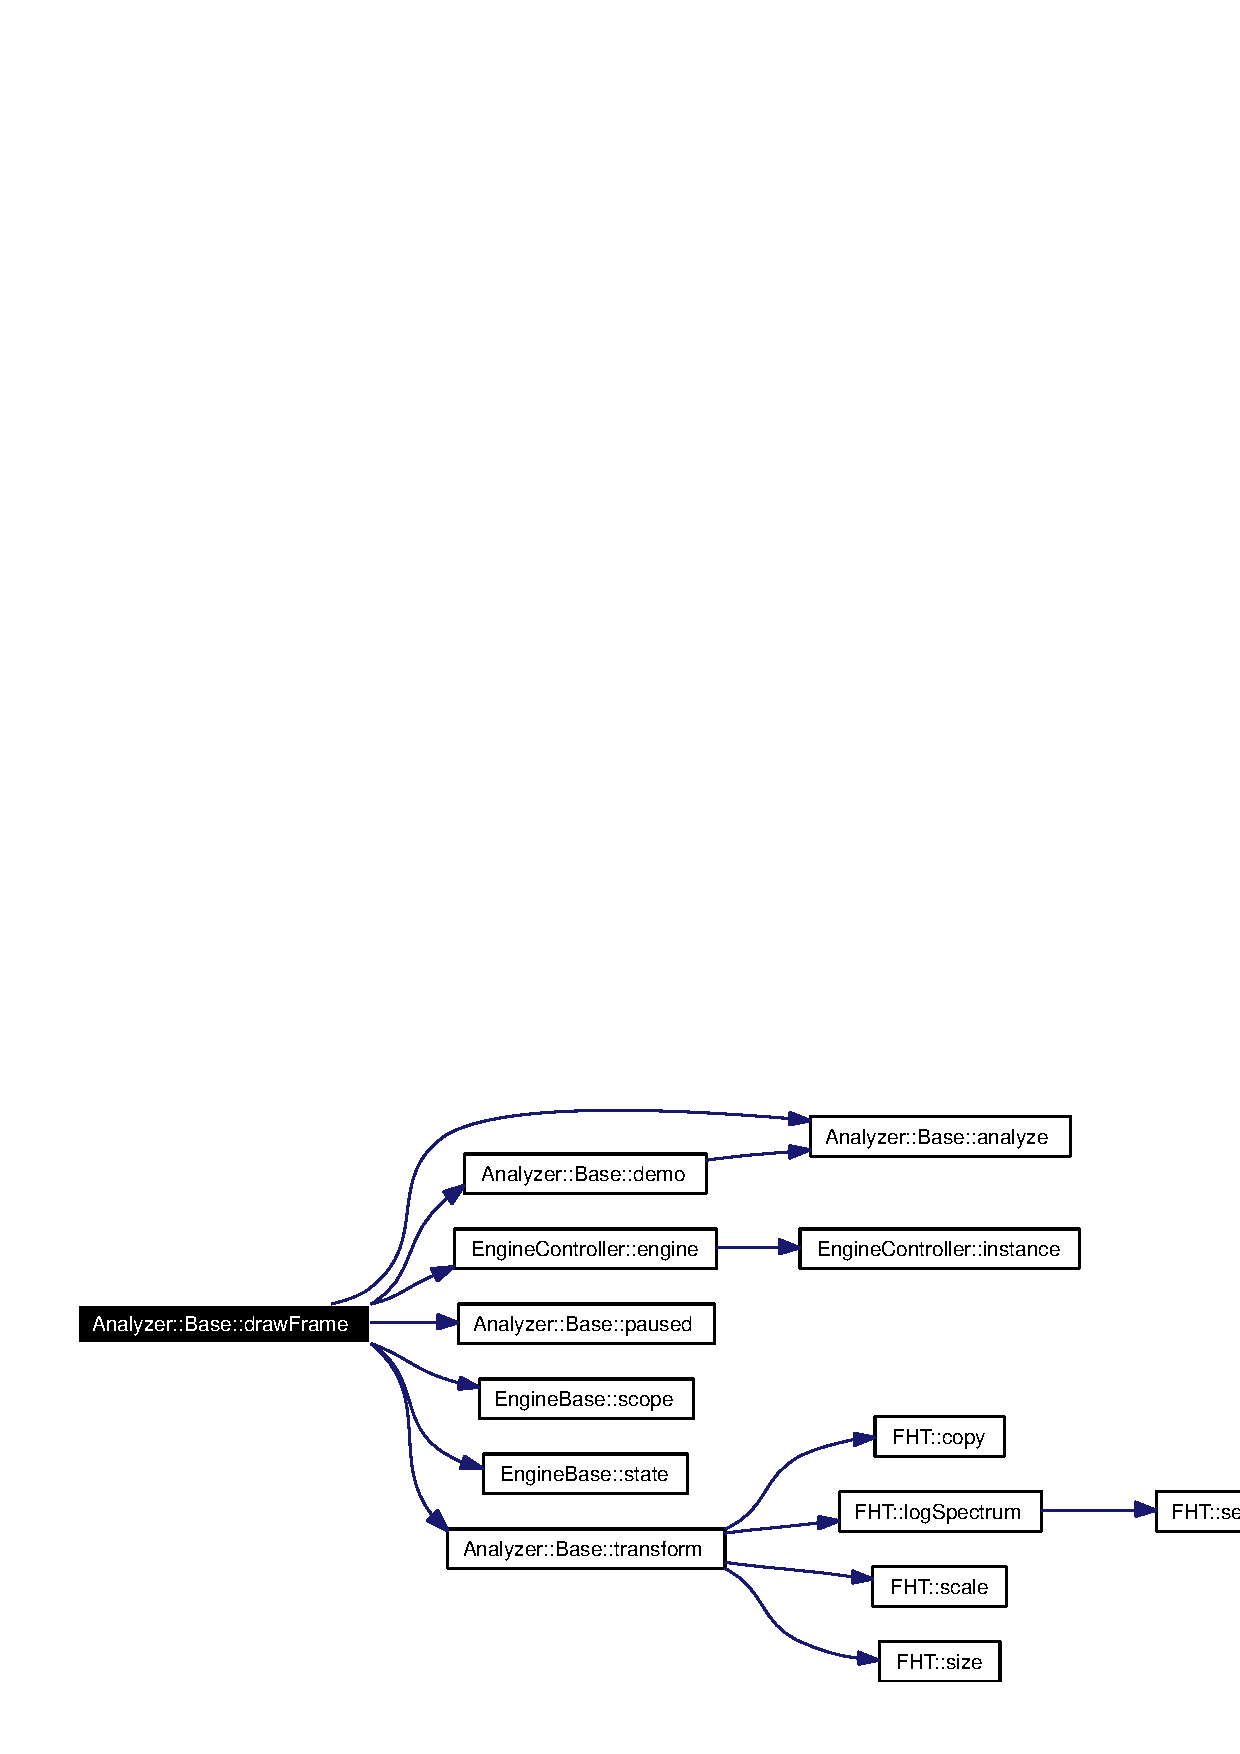
\includegraphics[width=393pt]{classAnalyzer_1_1Base_Analyzer_1_1Baseb1_cgraph}
\end{center}
\end{figure}
\index{Analyzer::Base@{Analyzer::Base}!event@{event}}
\index{event@{event}!Analyzer::Base@{Analyzer::Base}}
\subsubsection{\setlength{\rightskip}{0pt plus 5cm}template$<$class W$>$ bool {\bf Analyzer::Base}$<$ W $>$::event (QEvent $\ast$)\hspace{0.3cm}{\tt  [private]}}\label{classAnalyzer_1_1Base_Analyzer_1_1Based0}




Definition at line 51 of file analyzerbase.cpp.

References Analyzer::Base$<$ W $>$::m\_\-timer, and Analyzer::Base$<$ W $>$::timeout().



\footnotesize\begin{verbatim}52 {
53     switch( e->type() ) {
54 /*    case QEvent::Paint:
55         if( !canvas()->isNull() )
56             bitBlt( this, 0, 0, canvas() );
57         return true; //no propagate event*/
58     case QEvent::Hide:
59         m_timer.stop();
60         break;
61 
62     case QEvent::Show:
63         m_timer.start( timeout() );
64         break;
65 
66     default:
67         break;
68     }
69 
70     return QWidget::event( e );
71 }
\end{verbatim}\normalsize 


Here is the call graph for this function:\begin{figure}[H]
\begin{center}
\leavevmode

\includegraphics[width=156pt]{classAnalyzer_1_1Base_Analyzer_1_1Based0_cgraph}
\end{center}
\end{figure}
\index{Analyzer::Base@{Analyzer::Base}!height@{height}}
\index{height@{height}!Analyzer::Base@{Analyzer::Base}}
\subsubsection{\setlength{\rightskip}{0pt plus 5cm}template$<$class W$>$ uint {\bf Analyzer::Base}$<$ W $>$::height () const\hspace{0.3cm}{\tt  [inline]}}\label{classAnalyzer_1_1Base_Analyzer_1_1Basea1}




Definition at line 43 of file analyzerbase.h.



\footnotesize\begin{verbatim}43 { return m_height; }
\end{verbatim}\normalsize 
\index{Analyzer::Base@{Analyzer::Base}!paused@{paused}}
\index{paused@{paused}!Analyzer::Base@{Analyzer::Base}}
\subsubsection{\setlength{\rightskip}{0pt plus 5cm}template$<$class W$>$ void {\bf Analyzer::Base}$<$ W $>$::paused ()\hspace{0.3cm}{\tt  [protected, virtual]}}\label{classAnalyzer_1_1Base_Analyzer_1_1Baseb4}




Definition at line 124 of file analyzerbase.cpp.

Referenced by Analyzer::Base$<$ W $>$::draw\-Frame().



\footnotesize\begin{verbatim}125 {}
\end{verbatim}\normalsize 
\index{Analyzer::Base@{Analyzer::Base}!timeout@{timeout}}
\index{timeout@{timeout}!Analyzer::Base@{Analyzer::Base}}
\subsubsection{\setlength{\rightskip}{0pt plus 5cm}template$<$class W$>$ uint {\bf Analyzer::Base}$<$ W $>$::timeout () const\hspace{0.3cm}{\tt  [inline]}}\label{classAnalyzer_1_1Base_Analyzer_1_1Basea0}




Definition at line 42 of file analyzerbase.h.

Referenced by Analyzer::Base$<$ W $>$::event().



\footnotesize\begin{verbatim}42 { return m_timeout; }
\end{verbatim}\normalsize 
\index{Analyzer::Base@{Analyzer::Base}!transform@{transform}}
\index{transform@{transform}!Analyzer::Base@{Analyzer::Base}}
\subsubsection{\setlength{\rightskip}{0pt plus 5cm}template$<$class W$>$ void {\bf Analyzer::Base}$<$ W $>$::transform ({\bf Scope} \&)\hspace{0.3cm}{\tt  [protected, virtual]}}\label{classAnalyzer_1_1Base_Analyzer_1_1Baseb2}




Reimplemented in {\bf Sonogram} {\rm (p.\,\pageref{classSonogram_Sonograma4})}.

Definition at line 74 of file analyzerbase.cpp.

References FHT::copy(), FHT::log\-Spectrum(), Analyzer::Base$<$ W $>$::m\_\-fht, FHT::scale(), Analyzer::Scope, and FHT::size().

Referenced by Analyzer::Base$<$ W $>$::draw\-Frame().



\footnotesize\begin{verbatim}75 {
76     //this is a standard transformation that should give
77     //an FFT scope that has bands for pretty analyzers
78 
79     //NOTE resizing here is redundant as FHT routines only calculate FHT::size() values
80     //scope.resize( m_fht.size() );
81 
82     float *front = static_cast<float*>( &scope.front() );
83 
84     float* f = new float[ m_fht.size() ];
85     m_fht.copy( &f[0], front );
86     m_fht.logSpectrum( front, &f[0] );
87     m_fht.scale( front, 1.0 / 20 );
88 
89     scope.resize( m_fht.size()/2 ); //second half of values are rubbish
90     delete [] f;
91 }
\end{verbatim}\normalsize 


Here is the call graph for this function:\begin{figure}[H]
\begin{center}
\leavevmode
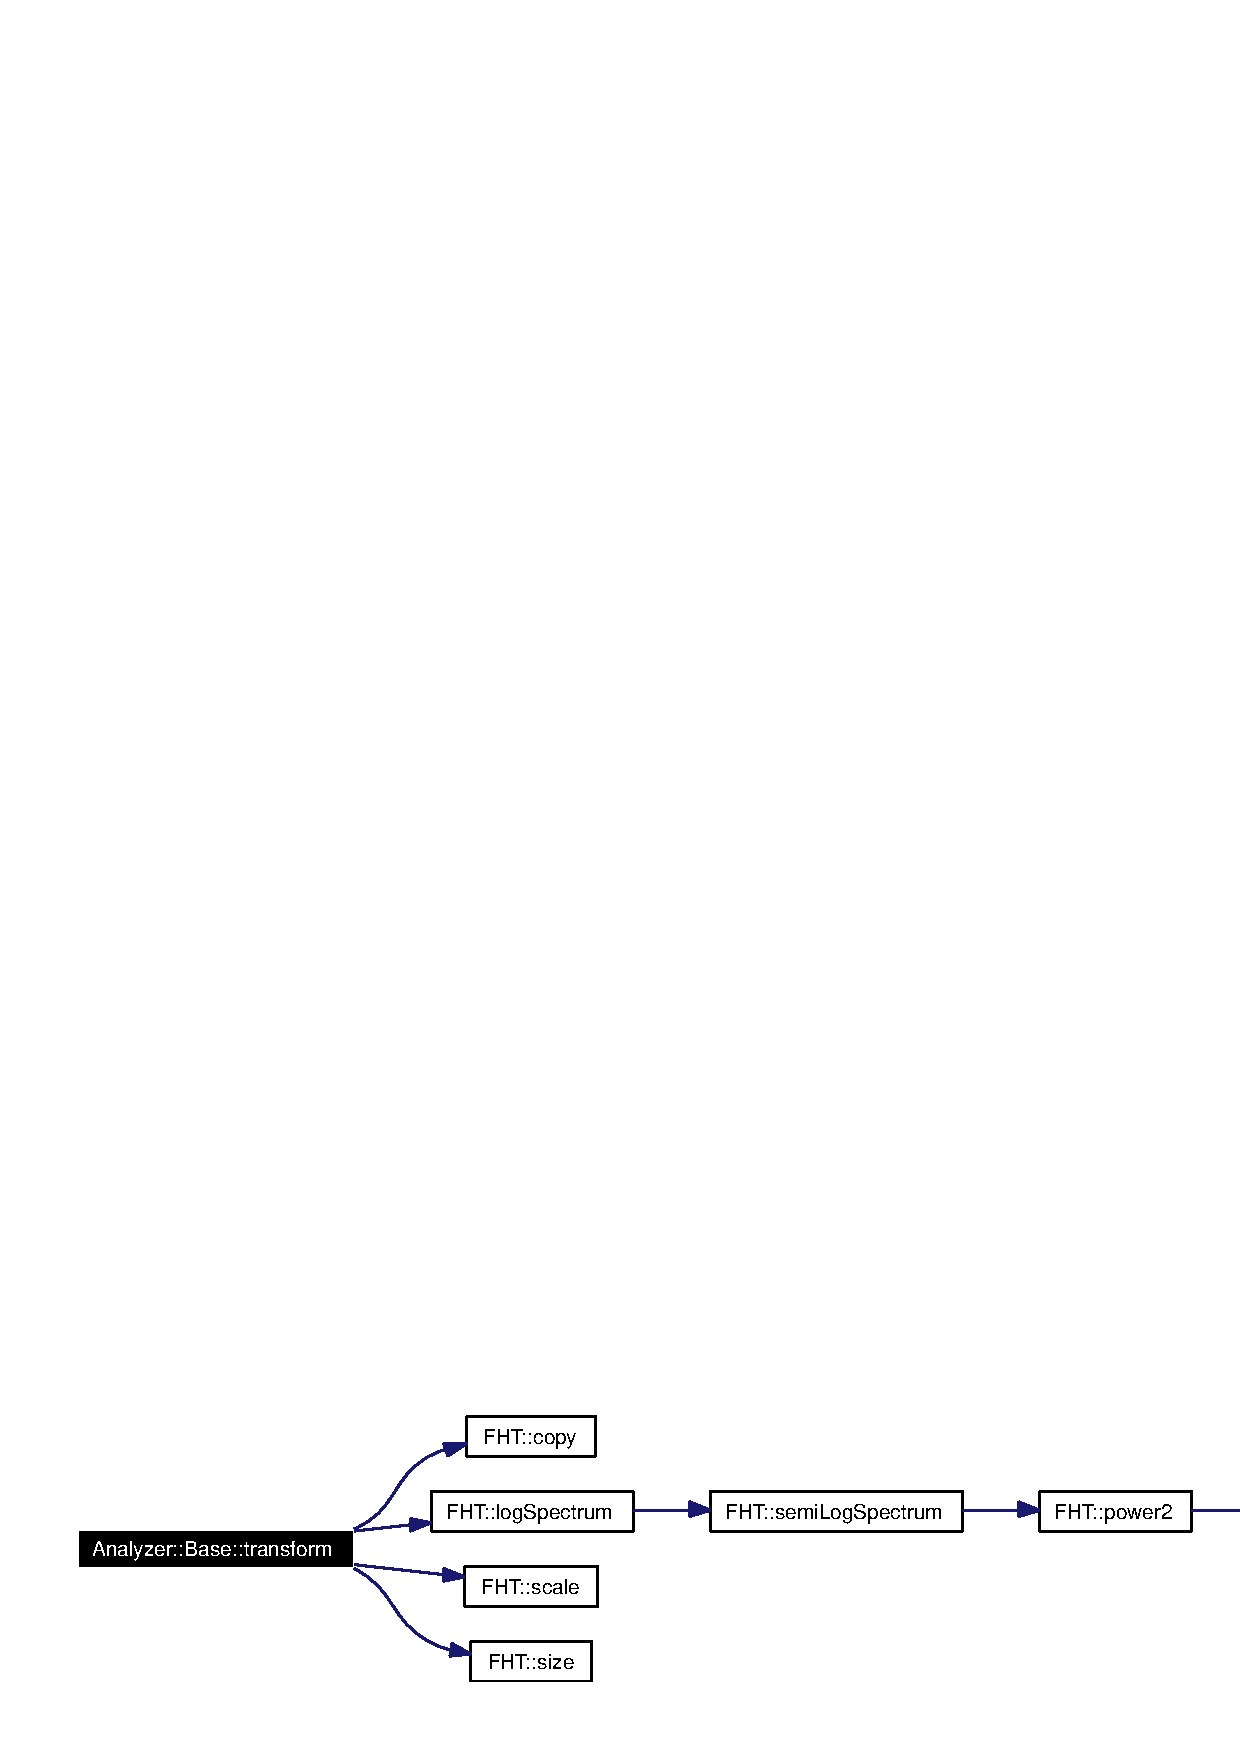
\includegraphics[width=349pt]{classAnalyzer_1_1Base_Analyzer_1_1Baseb2_cgraph}
\end{center}
\end{figure}


\subsection{Member Data Documentation}
\index{Analyzer::Base@{Analyzer::Base}!m_fht@{m\_\-fht}}
\index{m_fht@{m\_\-fht}!Analyzer::Base@{Analyzer::Base}}
\subsubsection{\setlength{\rightskip}{0pt plus 5cm}template$<$class W$>$ {\bf FHT} {\bf Analyzer::Base}$<$ W $>$::{\bf m\_\-fht}\hspace{0.3cm}{\tt  [protected]}}\label{classAnalyzer_1_1Base_Analyzer_1_1Basep3}




Definition at line 67 of file analyzerbase.h.

Referenced by Analyzer::Base$<$ W $>$::transform().\index{Analyzer::Base@{Analyzer::Base}!m_height@{m\_\-height}}
\index{m_height@{m\_\-height}!Analyzer::Base@{Analyzer::Base}}
\subsubsection{\setlength{\rightskip}{0pt plus 5cm}template$<$class W$>$ uint {\bf Analyzer::Base}$<$ W $>$::{\bf m\_\-height}\hspace{0.3cm}{\tt  [protected]}}\label{classAnalyzer_1_1Base_Analyzer_1_1Basep2}




Definition at line 66 of file analyzerbase.h.\index{Analyzer::Base@{Analyzer::Base}!m_timeout@{m\_\-timeout}}
\index{m_timeout@{m\_\-timeout}!Analyzer::Base@{Analyzer::Base}}
\subsubsection{\setlength{\rightskip}{0pt plus 5cm}template$<$class W$>$ uint {\bf Analyzer::Base}$<$ W $>$::{\bf m\_\-timeout}\hspace{0.3cm}{\tt  [protected]}}\label{classAnalyzer_1_1Base_Analyzer_1_1Basep1}




Definition at line 65 of file analyzerbase.h.\index{Analyzer::Base@{Analyzer::Base}!m_timer@{m\_\-timer}}
\index{m_timer@{m\_\-timer}!Analyzer::Base@{Analyzer::Base}}
\subsubsection{\setlength{\rightskip}{0pt plus 5cm}template$<$class W$>$ QTimer {\bf Analyzer::Base}$<$ W $>$::{\bf m\_\-timer}\hspace{0.3cm}{\tt  [protected]}}\label{classAnalyzer_1_1Base_Analyzer_1_1Basep0}




Definition at line 64 of file analyzerbase.h.

Referenced by Analyzer::Base$<$ W $>$::event().

The documentation for this class was generated from the following files:\begin{CompactItemize}
\item 
{\bf analyzerbase.h}\item 
{\bf analyzerbase.cpp}\end{CompactItemize}
